%; whizzy chapter -initex iniptex -latex platex -format platex -bibtex jbibtex -fmt fmt
%%%; whizzy chapter -advi -initex iniptex -latex platex -format platex -bibtex jbibtex -fmt fmt 
%   Pdf作成手順
% dvipdfmx 200502.dvi

%この資料は両面印刷で印刷すること


%     Tokyo Debian Meeting resources
%     Copyright (C) 2006 Junichi Uekawa

%     This program is free software; you can redistribute it and/or modify
%     it under the terms of the GNU General Public License as published by
%     the Free Software Foundation; either version 2 of the License, or
%     (at your option) any later version.

%     This program is distributed in the hope that it will be useful,
%     but WITHOUT ANY WARRANTY; without even the implied warranty of
%     MERCHANTABILITY or FITNESS FOR A PARTICULAR PURPOSE.  See the
%     GNU General Public License for more details.

%     You should have received a copy of the GNU General Public License
%     along with this program; if not, write to the Free Software
%     Foundation, Inc., 51 Franklin St, Fifth Floor, Boston, MA  02110-1301 USA


\documentclass[mingoth]{jsarticle}
\usepackage[dvipdfmx]{graphicx}
\usepackage[dvipdfmx]{hyperref}
\usepackage{fancybox}

%http://www.naney.org/diki/dk/hyperref.html
%日本語EUC系環境の時
\AtBeginDvi{\special{pdf:tounicode EUC-UCS2}}
%シフトJIS系環境の時
%\AtBeginDvi{\special{pdf:tounicode 90ms-RKSJ-UCS2}}

\newenvironment{commandline}%
{\VerbatimEnvironment
  \begin{Sbox}\begin{minipage}{12cm}\begin{tiny} \begin{BVerbatim}}%
{\end{BVerbatim}\end{tiny}\end{minipage}\end{Sbox}
  \setlength{\fboxsep}{8pt}\fbox{\TheSbox}}

\newcounter{santakucounter}
\newcommand{\santaku}[4]{%
\addtocounter{santakucounter}{1}

\nopagebreak 問題\arabic{santakucounter}. 
#1\\
\nopagebreak□ A #2\\
\nopagebreak□ B #3\\
\nopagebreak□ C #4
\pagebreak[1]
\hspace{1cm}
\\

}

\newcommand{\emptyspace}{(\underline{\hspace{1cm}})}


% sectionをセンタリングする
\makeatletter
  \renewcommand{\section}{\@startsection{section}{1}{\z@}%
    {\Cvs \@plus.5\Cdp \@minus.2\Cdp}% 前アキ
    {.5\Cvs \@plus.3\Cdp}% 後アキ
    {\normalfont\Large\headfont\raggedright\centering}} % style
\makeatother

% section の代わりの環境
\newcommand{\dancersection}[2]{%
\newpage
東京エリアDebian勉強会 2005
\hrule
\vspace{0.5mm}
\hrule
\hfill{}
\includegraphics[width=3cm]{image200502/openlogo-nd.eps}\\
\vspace{-4cm}
\begin{center}
  \section{#1}
\end{center}
\hfill{}#2\hspace{3cm}\space\\
\hrule
\hrule
\vspace{1cm}
}

\begin{document}

\begin{titlepage}

\title{第1回 東京エリア Debian 勉強会\\事前資料
\footnote{機密レベル public: 一般開示可能}}
\date{2005年2月19日}
\author{非営利個人 上川 純一\thanks{Debian Project Official Developer}} 
\maketitle

\end{titlepage}

\newpage
\tableofcontents

\dancersection{Introduction To Debian 勉強会}{上川 純一}

1回目のDebian勉強会へようこそ。
これからDebianのあやしい世界に入るという方も、すでにどっぷりとつかってい
るという方も、月に一回Debianについて語りませんか?

目的として下記の二つを考えています。

\begin{itemize}
 \item メールではよみとれない、もしくはよみとってられないような情報を情
       報共有する場をつくる
 \item まとまっていないDebianを利用する際の情報をまとめて、ある程度の塊と
       して出してみる
\end{itemize}

また、東京にはLinuxの勉強会はたくさんありますので、Debianに限定した勉強
会にします。Linuxの基本的な利用方法などが知りたい方は、他でがんばってくださ
い。
Debianの勉強会ということで究極的には参加者全員がDebian Packageを
がりがりと作りながらスーパーハッカーになれるような姿を妄想しています。

Debianをこれからどうするという能動的な展開への土台としての空間を提供し、
情報の共有をしたい、というのが目的です。
次回は違うこと言ってるかもしれませんが、御容赦を。

\subsection{講師紹介}

\begin{itemize}
 \item{山根さん} クレーマーです。日本人で一番多くDebian ProjectのBTS(バ
      グトラッキングシステム/問題管理システム)にバグを登録しているかもし
      れない。
 \item{上川 純一} Debian Developerです。
      元超並列計算機やっていて、
      今は音楽関係とか、気づいたらcannaとか。
      あと、pbuilderとか、libpkg-guideとか、Debianの品質向上目指してます。
\end{itemize}

\subsection{事前課題紹介}

1回目の事前課題は
「1年後のDebian」というタイトルで200-800文字程度の文章を書いてください。
というものでした。
その課題に対して下記の内容を提出いただきました。

\subsubsection{岩松 信洋}

1年後のDebianについて

{\tt *Debian全体として}

一番注目すべきなのは Sarge がリリースされているか?ということだと思う。
この調子ではリリースされていない可能性も高い。スケジュールもずるずると
遅れてるし。1ユーザーとしてはリリースされていることを信じたい。
また、この原因としてメンテナがちゃんとパッケージを管理してなかったり、
活動してなかったりしてるのが問題ということをよく見かけるので、ちゃんと
リリースされていたらこの辺は改善する動きがあり、もっと活発なメンテナや
デベロッパーが増えてると思う。
そして、対応アーキテクチャが増え、その中にSuperHがあると思う。

{\tt *自分の1年後Debianな生活}

パッケージのメンテナとしてDebianに貢献していたい。また、英語の勉強もか
ねて翻訳の方にも参加していたい。


\subsubsection{東村さん}

下記は課題です。
\begin{verbatim}
 1年後のdebian
 - debian
  - debian sargeのリリースからdebian本が出る
    sargeでdebianブームがさらに広まってほしい
  - sarge本が大量に出版されてほしい。
    (debian勉強会から出版!?)
  - debian勉強会は有名に!!出席者が倍増すればうれしい

 - 個人として
  - debianでのIPv6検証をしたい
  - Packageを作成できるようになりたい
  - BTSを使うようにする
  - 教えてもらう側から教えられる側になりたい
 - Webサーバを作り、自分なりのdebian情報を公開したい
\end{verbatim}

\subsubsection{Hideki Yamaneさん}

■リリース\\
 さすがに sarge はリリースされているでしょう。


■セキュリティ対応の面から\\
 より多くのセキュリティ勧告が発行されているでしょう。下手をすると1000の大台まで行くかもしれません。これだけ多くの数のセキュリティ勧告の発行には、多大な工数を必要とします。しかしながら、セキュリティチームという人的資源には限りがあり、彼らも会社に対してフルタイムで勤務している社員ではないため、どのようにしてそのリソース不足を補うのかを真剣に考え始める必要があるように思います。この問題は深刻です。
 また、このセキュリティ勧告にはチェック漏れが多く発生し、セキュリティアップデートによって「動かない」という事態がより出てくるでしょう。これは利用環境構成の多様化の問題に伴って指数関数的に増える問題です。特に kenrel についてはこの問題が多く付きまとうことになり、それが故にタイムリーに勧告を発行できないジレンマも発生します。この点に関する不満が大きくなるでしょう。

 これに対応するには、セキュリティ問題を事前に防ぐ「監査」がより重要な意味を持つように思います。その際には人的資源の問題から、より多くの自動チェックが必要とされるでしょう。しかし、自動チェックを行うにしてもどのように行っていくのか、実際行うとしたら upstream レベルでの対応を行わなければ意味が無いのではないか、などの問題点が残されています。

 良い点としては sarge のリリースによって、upstream とのバージョン間の差異が縮まることで security update の backport の手間が多少減ることでしょうか。php の例にもあるように、リリース期間が伸びることによって upstream との乖離が大きくなり、単純な patch で解決できない状況が生まれつつあったので、この点は喜ぶべきことだと思います。


■権利関連\\
 より多くのライセンス・特許・商標関連問題が山積みになるでしょう。ユーザ側が多少の手間をかけることによって解決できることも多いですが(Unofficial な deb を利用するなど)、これは一般のユーザにとっては敷居が高く、「不自由さ」を感じさせることになるでしょう。

 それとは逆に、今までライセンスの関係上導入が難しかった部分が一部ながらも解決されていくでしょう。これは特に Java に関して顕著になるかと思います。


■Debian 固有の l18n/l10n 問題は改善されていくでしょう。\\
 debconf や package description の母国語化の作業はほぼフレームワークが出来つつあり、あとは作業を進めるだけとなっています。問題は翻訳の質をどのようにたかめていくかですが、一般ユーザからのフィードバックをどのように迅速に適用するかが肝かもしれません。


■Quality の問題をどう解決していくのか\\
 多数のパッケージの集合体が Debian なわけですが、その質はさまざまです。この品質をどう上げていくのか、単なる packaging issue ではない、本当の意味での QA が求められるようになっていくと思われます。現状では、MIA の追跡から NMU の打診などが debian-qa では行われているようですが、実際に「質を上げる」という意味では機能していないようです。誰がどのようなパッケージを保持しててどんなバグを持っているのか、まではシステマチックに追いかけているようですが、実際にそのバグを潰す方法・もっと能動的に質を高めていく方法がそろそろ問われ始めるのではないでしょうか。


\subsubsection{Masakazu Takahashiさん}
1年後のDebian、ていうか自分

いま、あるソフトのちょっとしたバグを追いかけている。が、まだスキルがな
いため遅々として進まない。そこで、この1年ぐらいで、とりあえず自分しか
困らないようなバグでも自分で直せたり、またはバグレポートしたりできるよ
うにスキルアップしたい。そのためには、プログラム内容の理解はもちろん、
パッケージの作り方から、バグの原因を見つけるためのエスパー能力までいろ
いろ学びたい。

\subsubsection{なかじま きよたかさん}

1年後のDebian	
 1年じゃそんな変わらないと思うんだけどそんなことを書いてても面白くないので要
望みたいなの
を書きたい。
 今ケータイから書いているんだけど、とにかくパソコンみたいな端末にを使える余裕
がないので、
携帯端末で使えるのが欲しい。
 あと障害者用にカスタマイズされたのとかあればいいと思う。
 すべて音声で読み上げなどディスプレイ使わないですむのが理想だ。
 あとインストール済みの端末とかあるといいなぁ。
 というのでどうでしょうか。

\subsubsection{山本@戸塚さん}


現在我が家では、Debianはサーバ用OSとしての利用がほとんどという状態です。
私の1年後のDebianへの第一の期待は、デスクトップ用途としての使い勝手が
もう少しよくなってほしいということになります。

Debianへの期待というよりも現在のLinuxに対する一般的な要望ですが、まず、
Open Office がもう少し完成度が高くなってくれる(MS Officeとの互換性が
もう少しあれば...)と、助かります。ブラウザやメールに関しては、Mozilla 
が頑張ってくれているので、かなりよくなったと思います。あと一歩進めば、
私の仕事用のデュアルブートのLaptopも、Debianの起動時間がWindowsより長
くなるでしょう。

その他に、マルチメディア機能の充実が望まれます。現在もMP3ファイルのサー
バとして使っていますが、1年後にはいわゆる「メディアサーバ」として、音
楽、TV、DVD、ビデオ等のコントロールセンター(サーバとプレーヤー両方の
機能を提供する)として、居間で活躍してくれるとうれしいです。MythTVが
HDTVに対応するHDDレコーダーとして、気軽に使えるようになったらスゴイと
でしょう。あと、HD DVD再生機能も早めにほしいですね。

居間のTVモニターだけでなく、仕事場や台所のTVやパソコンでも無線LANで、
メディアサーバ上に貯めたコンテンツをいつでも楽しめるようになったら最高
ですね。

いまでも、スキルと時間があれば、これらの機能の多くががDebian上で実現で
きると思いますが、私が「1年後のDebian」に望むのは、CDイメージをインス
トールしたら、あとは設定ファイルをちょっといじるぐらいで、デスクトップ
機として、マルチメディア機として、使えるようになることです。

\subsubsection{松山さん}
携帯で自宅サーバにアクセスして録画予約したり,
湯水のようにディスクを浪費しつつスゴ録のような感じにしたりできてたらいいなぁとふと思いました.
...恥ずかしながら,動画のエンコードで挫折して1年程経過してます.
...まぁ,とにかく公私問わず明るく元気に「私,Debian使ってますけど?」と
言えるような社会になってたらよいかなぁと思います.
「あー,あなたもですか」などと自然に受け止められたら
もう言うことなしかと思いました.

\subsubsection{えとーさん}
「暗い1年後のDebian」

sarge 出るものの、RedHat、SuSeなどのリリースに押され
いまいち盛り上らない。

順調に日本の Debian Developer の平均年齢が一つ以上上り。
ますます日本の高齢化社会を体現していく、ML では調べることを
しない人により壊滅状態となり、情報を持っている人は日本の
debian-user,debian-devel などは見なくなる。

sargeは出たもののあいかわらずハードベンダーなどではサポートされず
一部のマニアのものとしてあつかわれ、ubuntulinux 社員の Debian developper が
会社の都合で恣意的にリリースを妨害したと大フレームが発生し評判を落した 
ubuntunlinux が倒産し「あぁ、やっぱりDebianに関わった企業は倒れるんだね」
と認識される。

就活で Debian 使ってます、と履歴書に書くと書類で弾かれるようになり
ますますユーザー、Developperが減り、一部のDebianユーザ達の集りは
ますます宗教の様相を呈し、「えー、Debian使ってるの?マニアックだなぁ」
と言われてた人が「え、、、Debian 使っているんですか、それは置いといて**」
とか、話題に上げることすら困難になる。

「明い1年後のDebian」

遅れに遅れていた sarge のリリースと共にHPなどが正式サポートを表明
ブレードサーバやクライアントなどでインストールする元となるマシンの量が激
増することによるライセンス費用の増大を避けるために続々と Debian を採用する
ユーザ企業が増大、企業で業務として Debian を触る人が増え、求人が拡大、
学生達もその流れに魅かれ続々と使用を始め、少ないながらもコミットを始める
10代の若者が増えるようになり、企業も徐々のではあるが、コミットを始めることとなる。
それにより l10n 活動も活性化しあらゆるツールが母国語で不便なく利用可能となる。

spam BTS を効率的にフィルタリングするように BTS システム が改善され、効率的にバグの
報告や修正などが可能となり、放置されるバグは続々と解消されていき、
構成管理などに便利なツールも増え Debian ユーザはますます堕落を謳歌する
黄金時代の始まりを予感している。

とか、二つのストーリーを考えてみました。w

\subsubsection{立神梢一さん}

これはDebianに限ったことではないかもしれないが、実際のところ個人でのLinuxの
導入の敷居は
実際はまだまだ低いものとはいえない。
各種商用ベンダーがデスクトップ戦線で苦戦し、結局Enterprise用途や、企業などで
の端末へ用いる
為のデスクトップパッケージへ注力しているのも、どうしてもまだまだWindowsの牙
城を崩せないからではないだろうか。
実際のところ、自分もいまだ主要デスクトップはWindowsである。
そこで、まずは自分の主要環境の脱Windowsを1年後には果たしたい。
本当はもっと早期に行いたいのだが、やはり既存の資産(というほどたいしたもので
はないが)
や、慣れの問題もあってなかなか難しいところもあるのだが、しかしいくら
Linux/UNIXへ傾倒していても
自分の使っているデスクトップがWindowsでは、個人的な美意識の問題から「カッコ
ワルイ」のだ。
それに加え、自分が主要デスクトップ機をLinuxへシフトする段階で、ドキュメント
的な部分への貢献ができれば
と考えている。
開発/プログラミング的な部分への貢献ができれば一番良いのだろうが、正直なとこ
ろ、自分自身がコンピューター
そのものへ興味をもった年齢が遅すぎたこともあり、また現在の自分の興味や仕事の
ベクトルと若干ずれる部分も
あるため、やはりドキュメンテーションや、いいとこテスターというか試用してバグ
報告するのが関の山だろう。
ともかくも1年後には自分の主要デスクトップをLinux化し、その過程でDebianを布教
(?)して行きたい。
あんまり壮大な計画ではないが着実な目標を、今回はあげてみました。1年後には
Sargeが安定版になっているんでしょうか。
「1年後のDeiban」というより「1年後にDebian」になってしまいました。以上です。

\subsubsection{三島さん}

【一年後の Debian】(一年後の視点から…)

1. sarge が出ました。

2. sarge の反省を元に、「もーちょっとまともにリリースマネジメント
   やったほうがよくね?」という議論が出ました。現在も議論中です。

3. パッケージにPGP証明書がつき、P2Pによる再配布が標準的になりました。

4. ソースからパッケージをビルドするのが容易になりました。いくつかの
   アプリケーションで劇的な最適化が。

5. ○○市の市役所の OS に採用されました。××銀行はATMへの搭載を
   進めています。あと、ローソンのロッピーにも載りました。

6. xfree86 → x.org と移行しました。ついでに標準デスクトップが
   Looking Glass になりました。

7. 次のプロジェクトが立ち上げられました (が、リリースされないと
   思います) : Debian GNU/MacOS, Debian GNU/OpenSolaris .

8. Debian GNU/Hurd がついに公式リリースされました。
   あと Debian GNU/kFreeBSD も。

9. 国際化についてはより進化しました。コンソールに IM が付きました。
   長年の問題だった、初期状態のコンソールで日本語が出力されない件に
   対しては、ローマ字ロケールが新たに作成されることによって対応
   されました。


\subsubsection{三塚@美紗緒ネットワークさん}

1年後のDebianということで、夢を語らせていただきたいと思います。

現在のDebianは、stableのリリースが遅いという評判があり、その結果
unstableに人が集まってしまっているという問題があるかと考えています。

本来、unstableは現在のexpermentalのような位置づけであったと思いますが
それがいつの頃からかtestingのような役割を果たすようになってしまって
いるかと思います。
これは何故かというと、stableのリリースを促進するために導入されたはずの
testingの機構が、逆にtesting離れを引き起こし、その結果としていつまでも
testingが成熟せずstableがリリースできないという人離れスパイラルを
引き起こしているからではないでしょうか?
現在のtestingは、unstableから機械的にパッケージが導入されてしまうため
頻繁に依存関係が崩壊して常用するのが難しいとの評判です。

そこで、今後の対策としてtestingを常用できる状態にすべく、パッケージ選定に
新しいルールを追加してみてはどうでしょう。
例えば、testingのパッケージに重大なバグが発見された場合、BTSに登録する
ことで即座にunstableから新しいパッケージが導入されるような仕組みです。
testingの品質が上がることでtestingを常用するユーザーが増え、それがさらに
品質のアップに繋がり、という良い連鎖になっていくといいなと思います。



\subsubsection{上川}

一年後のDebian Projectは、
やっとsargeをリリースし、一段落して、これからどうするか、ということを検
討しはじめるステージにでてきているでしょう。

これから実施したいのは、よりリリースプロセスに統合化されたテストのシステ
ムです。
労力を省略するために自動化したテストをはしらせ、それらをBTSなどのトラッ
キングシステムと統合します。

現状はテストを走らせ、その問題を全て解決するというフローに人の手が介在し
すぎており、人のリソースが有効に利用できていないという問題があります。

一部の人間だけが知っているシステム、一部の人間だけが知っている問題、
というものがリリースを遅れさせることは今回のsargeリリースで明確になって
きたと思います。これからは、できるかぎり一般的な部分については、一部の人が
居なくなってもそれなりにまわるようにインフラを作り変えたいと考えています。


%%% trivia quiz
\dancersection{Debian Weekly News trivia quiz}{上川 純一}

ところで、Debian Weekly News (DWN)は読んでいますか?
Debian 界隈でおきていることについて書いているDebian Weekly News.
毎回読んでいるといろいろと分かって来ますが、一人で読んでいても、解説が少
ないので、
意味がわからないところもあるかも知れません。みんなでDWNを読んでみましょう。

漫然と読むだけではおもしろくないので、DWNの記事から出題した以下の質問にこたえてみてください。
後で内容は解説します。


\subsection{2005年2号}

\santaku{KDE 3.3がtestingにはいるために必要だったのはなにか
}{地の理}
{Britneyの手動操作}{天候}

\santaku{Gccに含まれているJava VMはどれか
}{Kaffe}
{Gij}{JamVM}

\santaku{バイナリファームウェアを別途ディスクなどからロードするように実
装しなおしたカーネルのデバイスドライバについて問題となっているのは何か
}{フリーではないものを必要とするものはcontribにはいるべきだが、カーネル
はcontribにはいるべきなのか}
{カーネルにディスクアクセスをさせたくない}{ディスクからファームウェアを
読み込むようにする機構を作成するのは不可能}


\santaku{debhelperを使わないでパッケージを作る方法について
のメールが流れたのはどのメーリングリストか。
}{debian-mentors}
{debian-devel}{debian-women}


\santaku{Joey HessがこのChangelogのエントリはひどいだろう、と指摘したの
は
}{下らないジョーク}
{女性蔑視な文面}
{学生が課題で提出した内容について「あそこの学生は最近はダメだな」と言及
したもの}


\subsection{2005年3号}

\santaku{中国でのDebian miniconfはいったいどこで行われるか
}{Beijing}
{Pyongyang}{Seoul}

\santaku{2004年にPorto Alegreで実施したdebconfの参加者は
}{53}
{163}{1000}


\santaku{LCA Mini-Debconf はどこで実施される?
}{Australia}
{Akasaka}{Austria}


\santaku{起動時にデーモンを起動しなくする設定をアップグレードした後も変
更されないようにする方法として間違っているのは?
}{update-rc.d -f service removeでシンボリックリンクをすべて削除する}
{/etc/init.d/serviceスクリプトの最初にexit 0 を挿入する}{invoke-rc.dのpolicy-rc.dをいじる}

\santaku{graphvizは関連図などを作成するのにしばしば使われているソフトウェ
アですが、最近何が起きた?
}{やっとDFSG-freeになった}
{革新的にユーザにとって使いやすくなった
}{vcg にのっとられた}


\santaku{debian/copyrightファイルについて、ライセンスを正確に記述しよう、
全ての著作権者の一覧を作成しようというメールを書いたのは
}{Branden Robinson}
{Jochen Voss}{Henning Makholm}

\subsection{2005年4号}

\santaku{volatile woodyに追加された最初のパッケージは?
}{amavis}
{spamassassin
}{whois}

\santaku{DevFSに大きく依存して実装しているdebian-installerの
開発チームに大きな衝撃を与えたのが、linuxカーネルからのDevFSの削除。
それが予定されている時期は
}{2005年7月}
{2005年2月
}{2099年9月9日}

\santaku{1月16日のDebian Women IRCミーティングで決定した事項は
}{存在感をあたえつつdebian 全体をおどしているようには見えないように頑張
る}
{Debian Projectへのねずみ講形式の女性勧誘
}{Debian Projectからの男性の排除}

\santaku{root以外のユーザが直接/sbin/haltを実行するために必要な手順は
}{ln -sf /bin/true /sbin/halt}
{dpkg-statoverride --add root root 02755 /sbin/halt
}{chmod 02755 /sbin/halt}

\santaku{Mozilla Foundationとトレードマークについて同意した内容はどの観点で不足なのか
}{金銭的に問題が発生している}
{DFSG のLicense Must Not Be Specific To Debianに該当する
}{宗教的に受け付けられない条件になっている}


\subsection{2005年5号}

\santaku{MySQLパッケージの変更によって、大きな問題が予想されるものは何か
}{mysqlのデータベース自体の互換性が無い}
{mysqlのライブラリのABIとsonameが変更したために発生する大がかりな再コン
パイル作業とそこで現れる問題
}{コンパイラーのバグ}

\santaku{sargeのリリースノートはwoodyからのアップグレードをどのようにす
ることを推奨しているか。
}{aptitudeを使って実施すること}
{アップグレードを開始するまえに祈りをささげること
}{アップグレードできなくてもめげないこと}

\santaku{DebianのArchiveが正当であることをある程度証明できる経路を提供す
るために作られている、Archiveのgpg キー。
最近何がおきたか
}{Keyがexpireしたので作り直した}
{みんなが活用しはじめた
}{apt-getがサポートはじめた}


\santaku{問題がなかなか解決しないため、リリースの障害となっているので、
一時的にsargeのリリース対象から
除外されたアーキテクチャはなにか
}{m68k}
{sh}{mipsel}

\subsection{2005年6号}


\santaku{前Debian Project Leaderの娘で、今度Tuxracerについて発表する講演
者の名前はElizabeth Garbee だが、何歳からdebianをつかっていたか。
}{9}
{10}{23}

\santaku{FTPを利用しないでDebianパッケージをアップロードする方法は何があ
るか
}{FTPサーバのセキュリティーホールをさがし、そこからシェルアカウントを取得してcat}
{gluckのDELAYEDキューにsshでアップロード}{
alioth経由でアップロード}

\santaku{カーネル2.6.8をデフォルトにし、2.6.10をデフォルトのカーネルに設定できないと判断した理由
}{2.6.10がsparcで動作しない}
{2.6.10になるとIA64のシリアルポートの扱いが変更になる}{
d-iは現在2.6.8で動作しているから}
% すべて理由なんだけど、2.6.10が今回判断の基準になった。 I/Oが遅いという話しもあったが?


\santaku{パッケージがたくさんあって問題だと言われているNEWキューとは
}{OVERRIDEの編集が必要な変更がされたパッケージに対して、FTP-masterが手動
で操作する必要があるが、その未
処理のバックログのこと}
{新しいパッケージの一覧のこと}{
リリースに関係ないパッケージの一覧のこと}


\santaku{chownで指定するのに利用するユーザ名とグループ名の区切り文字は
}{:}
{。}{
/}

\subsection{2005年7号}


\santaku{Joerg JaspertがDAMとして発表したのは
}{Emeritus状態のデベロッパーに対してはNM処理に近いものをDAMが直接
実施します}
{Emeritus状態のデベロッパーはいつでももどりたいときに何の処理も必要なく
Debian Developerにもどれます}{
GPG キーはAdvocateさえ署名していればよいです}

\santaku{udevを利用している場合 /.dev ディレクトリを削除してもよいのか
}{本物の/devがそこにマウントされているため、システムが起動しなくなる}
{/.devなんか必要ないので、消してしまってよいです}
{むしろ/procをアンマウントしてください}

\santaku{cvsではなくsvkを利用して/etcをメンテナンスする利点でないものは
なにか
}{シンボリックリンクを扱えるバージョンシステムであること}
{CVS/等の特殊な管理用のディレクトリが生成されない}{
将来おきるだろう設定変更が予測できる
}

\dancersection{最近のDebian関連のミーティング報告}{上川 純一}

\subsection{東京エリアDebian勉強会0回目報告}

	  0回目勉強会の参加者は21人でした。
	  受付は松山さんにお願いしました。ちょっと分かりにくかったかも。
	  個人で会場は借りていたので、
	  建物の入ったところにあった案内板には「上川」とだけ書いてあったので、主催者の名前を
	  知らないとわからないですね。
	  会議室の前にあったホワイトボードにはDebian勉強会と(松山さんが)書いておきました。

最初は自己紹介から、参加者の方々がどのようなDebian生活を送っているのか赤裸々に語って頂きました。仕事でもDebianが使えているような結構凄い人が多いような。
	    初心者の方もきていらして、
	    この勉強会に参加するためにDebianを昨日インストールしてきました、昨日インストール失敗しました、昨日からサーバたってます、という方が複数名いらっしゃいました。


	    Debian勉強会で何をしたいのかという説明をしました。
	    目的としては、
	    MLとIRCとWEBだけの情報では情報交換に限りがあり、実際にface-to-faceで話しができる場所が欲しい、
	    というのと、
	    断片的な情報が多いのでまとまったドキュメントを生み出す場所としたい、という二点を説明しました。

	    Debian 関西新年会について報告しました。

	    Debian Weekly News Quizをしました。
	    3択の問題を12問出して、10分間で解いて頂きました。
	    答え合わせと解説をし、点数を調べた所、最高点数は11問正解のやまねさんでした。
	    記念品(?)を贈呈しました。
	    やってみておもしろかったのと、準備も楽なので、次もやろうかなと思います。

	    バックアップリストアについて上川が語りました。
	    会場からつっこみはいりまくりでした。
	    Debianで運用環境を構築している方が複数おられたので、
	    いろいろと有用な情報ありがとうございました。

	    ネットワーク機器監視について松山さんが語りました。
	    nagiosとか、設定の仕方が難しいのはどうだろう、という
	    話しで盛り上がっていました。
	    spongとか開発されているの?とか。


	    「来月はDebianの()に注目し、()なユーザをターゲットにしたその名も()勉強会を開催します。」
	    というお題で10分間で企画をそれぞれ考えて頂きました。
	    その後20分間5人グループ4つに分かれてグループの案を出していただき、
	    そして発表してもらいました。全員投票で一番よかったということになったのは、
	    「クレーマー養成講座」でした。
	    2ch とか blogとかに動かねえ、と一人でいっているのでは問題は解決しない、いったい
	    どういうクレームの出し方をすればDebianの改善までつながるか、ということについて
	    語るそうです。次回ぜひやって頂こうと言う事になりました。
	    チームには記念品を差し上げました、大切にしてあげてください。

	    個人で出して頂いた案については、上川が独断と偏見で選ばせて頂きました。
	    江藤さんの案「魔窟対談」、各デベロッパーの方々にdebianのなんだここは!という点を
	    あげてわいわいしてもらう、g新部さんと鵜飼さんで対決、とかしてみるとおもしろそう、
	    という案でした。
	    三島さんの案、「俺こんなの使っているぞ凄いだろ勉強会」の案は、
	    おたよりと称して、事前投稿されたマイナーパッケージについての
	    ネタを司会者が発表してみる、というものでした。
	    「某家の食卓」をイメージしているそうです。


	    懇親会は14人でぞろぞろと駅前の居酒屋で実施しました。
	    夜10時に開始して、気が付いたら午前3時、結局
	    9人くらいで、朝までDenniesに移動して過ごしました。
	    しんどい。。。もう歳か?
	    そのうちの一人は朝7時集合でスノーボードに行く、と言っていたのですが、大丈夫ですか?

	  今回0回目だから人が多かったのか、それとも次からは人が溢れ出てしまうのか、
	  今回の会場は21人でほぼ満員でした。定員は27人のはずです。
	  宴会場はつなげればおそらく30人くらいまでいけそうなので、
	  大丈夫かな?



\subsection{Washington D.C. Debian Developerたち}

\includegraphics[width=10cm]{image200502/washdc.eps}

Washington D.C. 在住の
Debian developer達に会って来ました。

二回ミーティングを開催して、
一度目はインド料理をたべてきました、
二度目は日本食を食べにいきました。

Washington D. C.
近辺に住んでいる人は政府系の仕事をしている人が多いという印象を受けました。


\subsubsection{Aaron M. Ucko}

最初に声をかけた主催者。
結婚していて、今1ヵ月半の子どもがいるとのこと。
奥様をつれてきておりました。

生物学の人達のためのプログラムの開発をして
生活しているそうな。
奥様は生物学の学生。


\subsubsection{Anthony DeRobertis}

若いDeveloper to be、おそらく22歳くらい。
まだDebian Developerにはなれていないとのこと。


\subsubsection{Patrick Ouellette}

写真にうつっている子どものお父さん。家族づれでした。

\subsubsection{Stephen Frost}

仕事も大変そうです。
キーを忘れて来たそうです。
もういっかいする際には忘れない、と言ってましたが、二度目には来れなかった
みたい。

%\subsubsection{Jay Berkenbilt}



\subsubsection{Robin Verduijn}

Washington D.C.に住んで居ながらみんな集まらないということを嘆いていまし
た。

\subsubsection{Joshua Juran}

Debianの人では特になく、classic MacOS上でposixを実装しているとか
言ってました。

\subsubsection{その他}

まだ居ましたが、全員とはお話しできませんでした。
訪問者が来ないと人が集まらないとかで、久しぶりにお互いに会ったようで、みなさん盛り上がってました。


\dancersection{debhelper論 その1}{Debhelperとは何か。存在意義は何か。}

\subsection{Debian packageの構成要件}


Debian Packageのソースパッケージには下記ファイルが必要です。
全てのファイルについては規定のフォーマットがあります。

\begin{itemize}
 \item debian/rules: パッケージをビルドする手順を記述したMakefile.
 \item debian/control: パッケージの情報を記述した構成ファイル
 \item debian/copyright: パッケージの著作権情報を記述したファイル。利用
       許諾を記述。
 \item debian/changelog: 変更履歴を記述する。
\end{itemize}


emacsで編集するのであれば、devscripts-elパッケージをインストールすると
編集しやすくなっています。
vi を利用しているのであれば、devscriptsパッケージを利用すると、
各ファイルを編集しやすいです。


パッケージの作成の本質は、ディレクトリ以下にアプリケーションをインストー
ルし、
それ以下のファイルをtarでかためて、debファイルのなかにいれることです。
その他に制御情報もありますが、それについては後日。

例えば、debian/tmp/以下に / 以下にインストールされるはずのファイルを配置
することでパッケージを作成できます。
debian/tmp/usr/bin/binary-test
というファイルを作成して、debian/tmpディレクトリを指定してdpkg-debコマン
ドを実行してできたパッケージをインストールしたら/usr/bin/binary-test
にファイルがインストールされます。


\subsection{dh-make}

アップストリームからのソースパッケージから、Debian用のパッケージのテンプ
レートを作成します。

さて、dh-make ではどんなファイルが作成されるのでしょうか。

なんでもないサンプルファイルを作成して試しに実行してみます。

\begin{commandline}
	
[02:11:56]ibookg4:/tmp/dh> find -ls 
 94712    0 drwxr-xr-x   3 dancer   dancer         80  1月 27 02:08 .
 94686    4 -rw-r--r--   1 dancer   dancer        156  1月 27 02:07 ./test-source_0.1.orig.tar.gz
 94672    0 drwxr-xr-x   2 dancer   dancer         60  1月 27 02:07 ./test-source-0.1
 94675    0 -rw-r--r--   1 dancer   dancer          0  1月 27 02:07 ./test-source-0.1/Makefile
\end{commandline}

dh-make コマンドをうつと、どんなバイナリを作成するのか、という点を聞かれ
ます。

\begin{commandline}
	
[02:13:42]ibookg4:/tmp/dh/test-source-0.1> dh_make

Type of package: single binary, multiple binary, library, or kernel module?
[s/m/l/k] s

Maintainer name : Junichi Uekawa
Email-Address   : dancer@debian.org 
Date            : Thu, 27 Jan 2005 02:13:46 +0900
Package Name    : test-source
Version         : 0.1
Type of Package : Single
Hit <enter> to confirm: 
Done. Please edit the files in the debian/ subdirectory now. You should also
check that the test-source Makefiles install into $DESTDIR and not in / .
[02:13:51]ibookg4:/tmp/dh/test-source-0.1> 
\end{commandline}


\begin{commandline}

[02:27:24]ibookg4:/tmp/dh/test-source-0.1> ls debian/
README.Debian  dirs		   manpage.sgml.ex  rules
changelog      docs		   manpage.xml.ex   test-source-default.ex
compat	       emacsen-install.ex  menu.ex	    test-source.doc-base.EX
conffiles.ex   emacsen-remove.ex   postinst.ex	    watch.ex
control        emacsen-startup.ex  postrm.ex
copyright      init.d.ex	   preinst.ex
cron.d.ex      manpage.1.ex	   prerm.ex
\end{commandline}

大量にファイルができます。これらのファイルで、.exで終了しているのはサン
プルファイルで、特に必要でないのなら削除します。


debian/rulesとして、次のようなファイルができます。

\begin{commandline}
#!/usr/bin/make -f
# -*- makefile -*-
# Sample debian/rules that uses debhelper.
# This file was originally written by Joey Hess and Craig Small.
# As a special exception, when this file is copied by dh-make into a
# dh-make output file, you may use that output file without restriction.
# This special exception was added by Craig Small in version 0.37 of dh-make.

# Uncomment this to turn on verbose mode.
#export DH_VERBOSE=1




CFLAGS = -Wall -g

ifneq (,$(findstring noopt,$(DEB_BUILD_OPTIONS)))
	CFLAGS += -O0
else
	CFLAGS += -O2
endif

configure: configure-stamp
configure-stamp:
	dh_testdir
	# Add here commands to configure the package.

	touch configure-stamp


build: build-stamp

build-stamp: configure-stamp 
	dh_testdir

	# Add here commands to compile the package.
	$(MAKE)
	#docbook-to-man debian/test-source.sgml > test-source.1

	touch build-stamp

clean:
	dh_testdir
	dh_testroot
	rm -f build-stamp configure-stamp

	# Add here commands to clean up after the build process.
	-$(MAKE) clean

	dh_clean 

install: build
	dh_testdir
	dh_testroot
	dh_clean -k 
	dh_installdirs

	# Add here commands to install the package into debian/test-source.
	$(MAKE) install DESTDIR=$(CURDIR)/debian/test-source


# Build architecture-independent files here.
binary-indep: build install
# We have nothing to do by default.

# Build architecture-dependent files here.
binary-arch: build install
	dh_testdir
	dh_testroot
	dh_installchangelogs 
	dh_installdocs
	dh_installexamples
#	dh_install
#	dh_installmenu
#	dh_installdebconf	
#	dh_installlogrotate
#	dh_installemacsen
#	dh_installpam
#	dh_installmime
#	dh_installinit
#	dh_installcron
#	dh_installinfo
	dh_installman
	dh_link
	dh_strip
	dh_compress
	dh_fixperms
#	dh_perl
#	dh_python
#	dh_makeshlibs
	dh_installdeb
	dh_shlibdeps
	dh_gencontrol
	dh_md5sums
	dh_builddeb

binary: binary-indep binary-arch
.PHONY: build clean binary-indep binary-arch binary install configure
\end{commandline}


また、debian/controlとして下記のようなファイルができます。

\begin{commandline}
Source: test-source
Section: unknown
Priority: optional
Maintainer: Junichi Uekawa <dancer@debian.org>
Build-Depends: debhelper (>= 4.0.0)
Standards-Version: 3.6.1

Package: test-source
Architecture: any
Depends: ${shlibs:Depends}, ${misc:Depends}
Description: <insert up to 60 chars description>
 <insert long description, indented with spaces>

\end{commandline}

他に必要なファイルとして、debian/changelogなどがあります。

\subsection{dh-xxxx のオーバビュー}

各論に入るまでにdh-xxxxが一般的にどういう動作を
するものなのかを説明します。おおざっぱにいうと二種類の動作形態があります。

Debian パッケージを作成する一連の動作の中で、
{\tt debian/パッケージ名 }
というディレクトリにインストール用のイメージを作成します。
そのディレクトリに対して、
{\tt debian/機能.パッケージ名 }
というファイルで指定した内容を実施してくれるのが
{\tt dh-機能} スクリプトです。

また、別の機能として、
コマンドラインオプションに指定されたものに対しても操作します。

\subsection{簡単なところから, dh-installman}

man ページをインストールするdh-installmanを例にとって、説明します。

man ページは各パッケージのセクションに応じたディレクトリにインストールし
ます。
セクション情報は、manページのroffソースの最初のところに記述してあります。

例\\

{\tt .TH "pbuilder" \underline{\it 8} "2004 Apr 4" "Debian" "pbuilder" }

このmanページはセクション8のマニュアルなので、FHSに従い、
{\tt /usr/share/man/man8/}というディレクトリにインストールする
必要があります。

下記の実行例は、インストール対象のパッケージ名を指定して、インストールす
るファイルを指定した場合です。

\begin{commandline}
 dh_installman -ppbuilder-uml pbuilder-user-mode-linux.1 \
 pbuilder-uml.conf.5 pdebuild-user-mode-linux.1
\end{commandline}

上記のコマンドを入力すると

{\tt debian/pbuilder-uml/usr/share/man/man1/pbuilder-user-mode-linux.1}
などにファイルがコピーされます。

debhelperの概念で重要なのは、このインストール先のディレクトリがどこであ
るかという
ことについてはdebhelper側で管理しており、
たとえポリシーに変更が発生しても、debhelperのみを変更すればよく、
パッケージスクリプト側への変更は最小にできる、という点です。

例えば、マニュアルページの例でいくと、
以前の標準では、/usr/man/man1/などにインストールすることがポリシーだった
のですが、それが変更になり、/usr/share/man/man1になりました。


\newpage
\vfill{}
\hfill{}

\includegraphics[width=7cm]{image200502/openlogo-nd.eps}
\hfill{}
\vfill{}
\newpage

\dancersection{個人提案課題}{}
\hfill{}{\large 名前} \underline{\hspace{6cm}}

下記の空欄を埋めてください:

{\LARGE 
来年までにはDebian の (\hspace{5cm})\\
に注目し(\hspace{6cm})なユーザを\\
ターゲットにした\\
その名も(\hspace{6cm})改革を実施します。
}
\\\\
企画案の図:

\newpage

\vfill{}
\hfill{}

\includegraphics[width=7cm]{image200502/openlogo-nd.eps}
\hfill{}
\vfill{}
\newpage


\dancersection{グループ提案課題}{}
{\large 名前} \underline{\hspace{6cm}} 
\hfill{}{\large 名前} \underline{\hspace{6cm}}

{\large 名前} \underline{\hspace{6cm}} 
\hfill{}{\large 名前} \underline{\hspace{6cm}}

{\large 名前} \underline{\hspace{6cm}} 
\hfill{}{\large 名前} \underline{\hspace{6cm}}\\

下記の空欄を埋めてください:

{\LARGE 
来年までにはDebian の (\hspace{5cm})\\
に注目し(\hspace{6cm})なユーザを\\
ターゲットにした\\
その名も(\hspace{6cm})改革を実施します。
}
\\\\
企画案の図:

\newpage
\vfill{}
\hfill{}

\includegraphics[width=7cm]{image200502/openlogo-nd.eps}
\hfill{}
\vfill{}
\newpage

\dancersection{Keysigning Party}{上川 純一}


事前に必要なもの
\begin{itemize}
 \item 自分の鍵のfingerprintを書いた紙
 \item 写真つきの公的機関の発行する身分証明書、fingerprintに書いてある名前が自分の
ものであると証明するもの
\end{itemize}

キーサインで確認する内容
\begin{itemize}
 \item 相手が主張している名前の人物であることを信頼できる身分証明書で証明し
       ているか\footnote{いままで見た事の無い種類の身分証明書を見せられ
       てもその身分証明書の妥当性は判断しにくいため、学生証明書やなんと
       か技術者の証明書の利用範囲は制限される。
       運転免許証明書やパスポートが妥当と上川は判断している}。
 \item 相手がfingerprintを自分のものだと主張しているか
 \item 相手のfingerprintに書いてあるメールアドレスにメールをおくって、
       その暗号鍵にて復号化することができるか
\end{itemize}

手順としては
\begin{itemize}
 \item 相手の証明書を見て、相手だと確認
 \item fingerprintの書いてある紙をうけとり、これが自分のfingerprintだと
       いうことを説明してもらう
 \item (後日) gpg署名をしたあと、鍵のメールアドレスに対して暗号化して送付、相手
       が復号化してキーサーバにアップロードする
\end{itemize}




\dancersection{次回}{}

次回は会場の都合などもあり、
3月13日日曜日の朝を予定しています。そんな時間に何人これるのか心配です。
内容は本日決定予定です。

参加者募集はまた後程。


\end{document}